\documentclass{physlab}
\usepackage{ctable}

%\newenvironment{bottompar}{\par\vspace*{\fill}}{\clearpage}

\begin{document}
\begin{titlepage}
\center % Center everything on the page
 
%----------------------------------------------------------------------------------------
%	HEADING SECTIONS
%----------------------------------------------------------------------------------------

\textsc{\LARGE Московский\\[-0.2cm]Физико-Технический Институт\\[0.1cm]\large (государственный университет)}\\[1.5cm] % Name of your university/college
\textsc{\Large Кафедра общей физики}\\[0.1cm] % Major heading such as course name
\textsc{\large Лабораторная работа № 3.1.1}\\[0.5cm] % Minor heading such as course title

%----------------------------------------------------------------------------------------
%	TITLE SECTION
%----------------------------------------------------------------------------------------

\HRule
\\[0.6cm]
{ \huge \bfseries Магнитометр}
\\[0.3cm] % Title of your document
\HRule
\\[1.5cm]


 
%----------------------------------------------------------------------------------------
%	AUTHOR SECTION
%----------------------------------------------------------------------------------------

\begin{minipage}[t]{0.48\textwidth}
	\begin{flushleft} \large
		\textsf{Студент}\bigskip
		
		\tline{(имя)}{30mm} \tline{(фамилия)}{45mm} \\[5mm]
		\underline{\hspace{30mm}} группа
	\end{flushleft}
\end{minipage}
\hfill
\begin{minipage}[t]{0.48\textwidth}
	\begin{flushright} \large
		\textsf{Преподаватель}\bigskip
		
		\tline{(имя)}{30mm} \tline{(отчество)}{45mm} \\[5mm]
		\tline{(фамилия)}{45mm}
	\end{flushright}
\end{minipage}

\begin{bottompar}
	\begin{center}
		
\includegraphics[width = 80 mm]{logo.jpg}
	\end{center}
	\tline{(дата)}{80mm}

\end{bottompar}
\vfill % Fill the rest of the page with whitespace

\end{titlepage}
	
	\paragraph{Цель работы:} определить горизонтальную составляющую магнитного поля Земли и установить количественное соотношение между единицами электрического тока в системе СИ и абсолютной гауссовой системе.
	\paragraph{В работе используются:} магнитометр, осветитель со шкалой, источник питания, вольтметр, электромагнитный переключатель, конденсатор, намагниченный стержень, прибор для определения периода крутильных колебаний, секундомер, рулетка, штангенциркуль
	\section*{Задание 1.}
	\subsection*{Экспериментальная установка}
	\begin{figure}[h]
		\begin{minipage}[h]{0.5\linewidth}
			\center{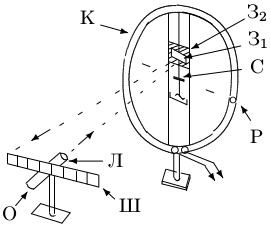
\includegraphics[width=0.5\linewidth]{station.png} \\ a) Схема магнитометра}
		\end{minipage}
		\begin{minipage}[h]{0.5\linewidth}
			\center{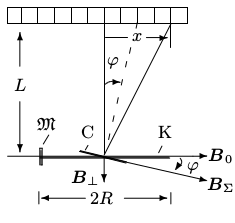
\includegraphics[width=0.5\linewidth]{station2.png} \\ б) Схема измерения угла
				отклонения магнитной стрелки}
		\end{minipage}
		\caption{Устройство магнитометра}
		\label{ris:station}
	\end{figure}
	Магнитометр — прибор для магнитных измерений — это компас, теодолит,веберметр и пр. С помощью магнитометров измеряют намагниченность ферромагнетиков, напряжённость магнитных полей, исследуют магнитные аномалии.\\
	\paragraph{Постановка задачи.} Измерим угол отклонения магнитной стрелки в поле намагниченного стержня и период колебаний этого стержня в поле Земли. По результатам измерений рассчитываем горизонтальную составляющую магнитного поля Земли.
	\paragraph{Выполнение измерений.} В нашей установке магнитную стрелку заменяют сменяют смещения двух световых зайчиков относительно друг друга. Вставляя намагниченный стержень в отверстие P (Рис.~\ref{ris:station}а) измерим смещение подвижного зайчика $x_1$ (Рис.~\ref{ris:station}б). Поменяв ориентацию стержня измерим $x_2$. Измерим расстояние от шкалы до зеркала $L$\\
	\[
	x1=\val
	\]
	\[
	x2=\val
	\]
	\[
	L=\val
	\]
	Опустим стержень на длинной нити в стеклянный сосуд, и измерим период его колебаний.
	\begin{table}[H]
		\centering
		\caption{Зависимость времени от колебаний}
		\begin{tabular}{|c|c|c|c|c|c|}
			\hline
			$t$, с & \val & \val& \val& \val& \val   \\ \hline
			$N$, колебаний & \val &\val  &\val  &\val  &\val    \\ \hline
			$T$, с & \val & \val& \val& \val& \val\\ \hline
		\end{tabular}
	\end{table}
	Получаем средний период колебаний $T_\text{ср.} = \val$.\\
	Измерим линейные размеры стержня
	\begin{align*}
	 m &= \val \\[1ex]
	 d &= \val \\[1ex]
	 l &= \val 
	\end{align*}Также нам был дан радиус кольца К (Рис.~\ref{ris:station}а) $R=\val$.\\ 
	Приведем основные погрешности измерений:
	
	\begin{minipage}{0.5\linewidth}
		\begin{align*}
			\sigma_l &= \val \\[1ex]
			\sigma_r &= \val \\[1ex]
			\sigma_T &= \val 
		\end{align*}
	\end{minipage}
~
\begin{minipage}{0.4\linewidth}
		\begin{align*}
	\sigma_R &= \val \\[1ex]	
	\sigma_L &= \val \\[1ex]
	\sigma_{x_1} &= \val 
	\end{align*}
\end{minipage}

	Произведем рассчет момента инерции ферромагнитного стержня:
	\begin{align*} 
		J=\val \\[1ex] 
		\Delta J=\val 
	\end{align*}
	Теперь рассчитаем магнитное поле: 
	\begin{align*}
	B_0 &= \val \\[1ex] 
	\Delta B_0 &= \val
	\end{align*}	
	\section*{Задание 2.}
	%\subsection*{}
	Вынув намагниченный стержень из гнезда P, мы собрали электрическую схема (Рис.~\ref{im:station3}). Подадим на рабочую установку напряжение $U$. Замкнем ключ К и включим электровибратор. Напряжение не изменилось, а отклонение зайчика $x_1'$.Поменяем полярность ключа и проведем аналогичные измерения: $x_2'$, среднее значение $x$
	
	\begin{minipage}{0.3\linewidth}
		\begin{figure}[H]
			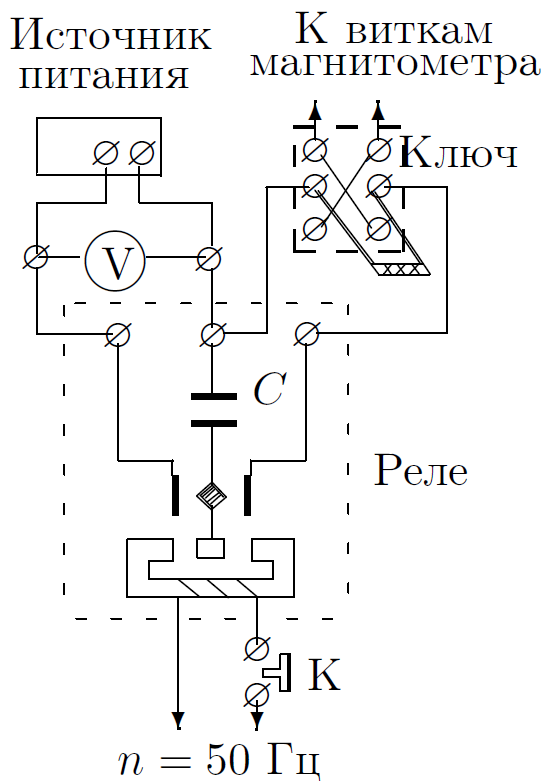
\includegraphics[width=50mm]{station3.png}	
			\caption{Схема питания катушки магнитометра}
			\label{im:station3}
		\end{figure}
	\end{minipage}
~
	\begin{minipage}{0.7\linewidth}
	\begin{align*}
		U &= \val \\[1ex]
		x_1' &= \val \\[1ex]
		x_2' &= \val \\[1ex]
		x &= \val
	\end{align*}
	Теперь рассчитаем силу тока в разных система СИ -- $I_{\text{СИ}}$ и в абсолютной гауссовой -- $I_\text{абс}$. \\
	Из параметров установки нам известно, что $N=\val$, рассчитаем tg$\,\varphi_2=\val$.\\ Получим:
	$$I_{\text{СИ}}=\val$$
\end{minipage}
	$$\Delta I_\text{СИ}=\val$$
	Для расчёта $I_\text{абс}$ переведем U в абс. гауссову систему\\ $U_\text{абс}= \val$, тогда:
	\begin{align*}
	I_\text{aбc} &=\val \\[1ex]
	\Delta I_\text{абс} &= \val  \\[1ex]
	c &= \val \\[1ex]
	\Delta c &= \val
	\end{align*}
	\large В итоге $c=\val$
	\section*{Вывод}
	 ~\\[-1ex]\hrule~\\[1ex]\hrule~\\[1ex]\hrule~\\[1ex]\hrule~\\[1ex]\hrule~\\[1ex]\hrule
\end{document}